\section{Open-Set Recognition}

Open-Set Recognition - метод распознавания с открытым набором параметров.
Порой может случиться так, что тестовый пример может быть визуально или метрически очень похожим на одну из категорий.
Наша задача - понять, когда эта кластеризация корректна, а когда мы делаем поспешные выводы.

\subsection{Основная идея}
Главной целью является попытка отличить похожие категории, которые были распознаны во время обучения, от новых, не идентифицированных. 
Другими словами, OSR специализируется на выявлении семантических сдвигов между категориями при обучении и тестировании.
Мотивацию можно представить как желание попытаться исключить ошибочное распознавание при близких параметрах, так как в реальном мире модели должны уметь не только различать объекты на существующих классах, но и идентифицировать случаи, когда сэмпл пришел из класса, который еще не встречался ранее.
Более инуитивное представление поможет получить картинка \ref{fig:anomalies-abstract}.

\begin{figure}[ht]
	\centering
	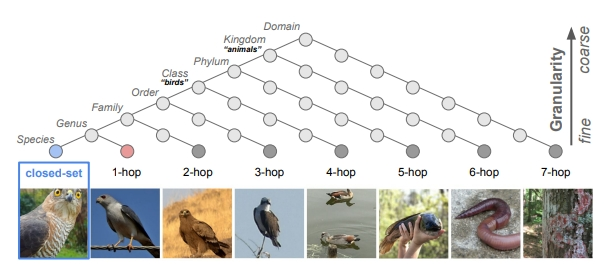
\includegraphics[width=0.8\linewidth]{chapters/anomalies/images/anomalies-abstract.jpg}
	\caption{Пример близких категорий из биологии}
	\label{fig:anomalies-abstract}
\end{figure}

На картинке мы видим, что чем дальше друг от друга виды животных на основе визуального восприятия, тем проще утверждать, что они относятся к разным классам и имеют более далеких предков.
Но чем ближе (пример - птицы), тем все труднее говорить о схожести видов, что может стать большой проблемой в силу некорректного отнесения животных к одному классу, роду или виду.
Иногда данная задача вызывает проблемы даже при попытке проделать ее самостоятельно, визуально.

\subsection{Постановка задачи}
Пусть у нас есть простанство объектов $X$, множество уже известных классов $Y = \{y_1, \dots, y_n\}$ и класс $u$ неизвестности, с которым мы как раз и должны научиться работать.

Модель в идеале должна сделать одно из двух следующих действий:
\begin{enumerate}
    \item Присвоить объекту $x \in X$ метку $y \in Y$, если объект принадлежит одному из известных классов.
    \item Присвоить метку $u$, если он не относится ни к одному из классов.
\end{enumerate}

\subsection{Методы}
\begin{enumerate}
    \item \textbf{На основе порога уверенности}
    
    Возьмем $S(x)$ за функцию, обозначающую отклик модели, он должен расти по мере роста $\mathcal{P}(y \in Y | x)$, где $y$ - предполагаемый класс объекта $x$. 
    Тогда:
    \begin{itemize} 
        \item Если $\max\limits_{y \in Y}{\mathcal{P}(y|x)}$ больше заранее определенного порога $\varepsilon$, то объект классифицируется моделью как принадлежащий $\hat{y} = \arg\max\limits_{y \in Y}{\mathcal{P}(y|x)}$.
        \item Если же меньше, то как неизвестный: $\hat{y} = u$
    \end{itemize}

    \item \textbf{На основе расстояний}
    
    Данный метод подходит если мы можем определить какую-либо метриуц на объектах.
    Метод основан на вычислении растояния от объекта до центров уже известных классов.
    
    Обозначим центры уже известных классов за $c_1, \dots, c_n$. 
    Обозначим за расстояние до центра $i$ за $d(x, c_i) = || x - c_i ||$. 
    Тогда:
    \begin{itemize}
        \item Если расстояние до ближайшего центра $cl(x) = \min\limits_{i}d(x, c_i)$ меньше заранее фиксированного порога $\varepsilon$, то объект классифицируется как принадлежащий $\hat{y} = \arg\min\limits_{i}d(x, c_i)$.
        \item Иначе же - как неизвестный: $y = u$.
    \end{itemize}
\end{enumerate}

По сути мы хотим минимизировать как количество ошибок классификации принадлежания одному из уже известных классов, так и отнесения к неизвестным объектам.
Стоит отметить, что при наличии явных выбросов или объектов, сильно отстояших от классов модель ложно отнесет их к неизвестным.

\subsection{Применение}
\begin{itemize}
    \item \textbf{Медицина}: распознавание и диагностика заболеваний, которые ранее могли быть еще не изучены или не встречаться
    \item \textbf{Биология}: пример с видами животных
    \item \textbf{Биометрия}: наверное самый наглядный пример, распознавание лица или отпечатка пальца человека. Мы должны сказать, является ли он известным или кто-то пытается взломать наш телефон
\end{itemize}

\subsection{Задачи}
Попробуйте ответить на следующие вопросы:

\problem Рассмотрим, как размер обучающей выборки для $n$ классов влияет на результат работы модели Open-Set Recognition. 
Формализуйте, как увеличение числа объектов в обучающей выборке может повлиять на вероятность ложных срабатываний и пропусков для неизвестных объектов.
\solution При небольшом размере обучающей выборки у модели не будет достаточной информации для точного определения границ между классами, что может привести к более высокому числу как ложных классификаций, так и ложных отнесений к неизвестному классу в силу отсутствия у нее возможности корректно научиться определять границы.

\problem Предложите метрику или способ обучения, которые вы бы использовали для оценки точности модели.
\solution С ходу понятно, как определять, что модель дала верный или не верный результат по уже известному классу. 
Но основная проблема состоит в том, чтобы оценить ее работу на объектах из неизвестного класса.
Давайте уберем из набора данных, используемого для тренировки часть, связанную с какими-либо известными классами, близкими к другим и будем валидировать способность нашей модели выделять неизвестные классы на ней.
Для оценки качества модели мы сможем применить метрику точности, равную отношению количества верных предсказаний в обоих случаях к общему количеству объектов:
$$Accuracy = \frac{TP + TR}{TP + TR + FP + FR},$$
где:
\begin{itemize}
    \item $TP$ - количество верных классификаций к одному из известных
    \item $TR$ - количество верных отнесений к неизвестному классу
    \item $FP$ - количество ошибочных кассификаций объекта как известного
    \item $FR$ - количество ошибочных отнесений объекта к неизвестным
\end{itemize}

\problem Предложите алгоритм, который можно было бы легко применить к задаче Open-Set Recognition.
\solution Давайте модифицируем логистическую регрессию. Для каждого класса $y_i$ она генерирует вероятность $\mathcal{P}(y_i|x)$, вычисляемую через сигмоидальную функцию.
Затем применим метод, основанный на пороге уверенности.

\section{Теория робастного (помехоустойчивого) обучения}
Традиционные методы обучения основываются на
том, что тренировочная выборка хорошо препроцессирована и не содержит шумов,
выбросов и недостающих значений. В реальных условиях хорошо структурировать
выборку не всегда возможно. В таких случаях на помощь могут прийти методы
робастного обучения.

Робастное обучение - это подход, фокусирующийся на построении моделей,
сохраняющих точность на неидеальных данных. Такая устойчивость обеспечивается
адаптивным подходам к входным данным. Методы обастного обучение частно
используют альтернативные функции потерь, алгоритмов, адаптирующихся к
структурам данных и/или детектирование и соответсвующую обработку аномалий.

\subsection{Схема итерационного взвешивания (IRS)}
IRS (Iterative Reweighting Scheme) - это один из
методов робасного обучения, заключающийся в обновлении весов объектов на каждом
шаге. Это позволяет уменьшить влияние аномальных данных. Вместо традиционных
функций потерь (таких как среднеквадратичная ошибка) в итерационной схеме
используются взвешенные функции потерь. IRS работает по следующему алгоритму:

\begin{enumerate}
  \item Инициализация весов
    Начинаем с иницаиализации весов:
    \[w_i^{(0)} = \frac{1}{l}, \forall i = 1, ..., l\]
  \item Обновление модели
    \[\alpha := arg min_{\alpha} \sum_{i=1}^l w_i L_i\left(\alpha\right) + \tau R\left(\alpha\right)\]

    \[w_i = norm_i\left( \mu^{'}\left( L_i(\alpha) \right) \right), i = 1, ..., l\]

    \[norm_i(v_i) = \frac{v_i}{\sum_j v_j}\]
  \item Повторяем обновление модели пока веса не стабилизируются или пока не
    будет достигнуто заданное число шагов
\end{enumerate}

\subsection{Задачи}
\subsubsection{Задача 1}
Предположим, что вы применили итеративную схему перевзвешивания на наборе
данных, содержащем выбросы. Вы применяете схему итеративного взвешивания.
По каким параметрам вы поймёте, чтоалгоритм сошёлся?
\textit{Ответ}: Веса изменяются не сильно, функция потерь перестала существенно
изменяться.
\subsubsection{Задача 2}
Предположим, что вы применили схему итерационного перевзвешивания к набору
данных и получили следующие веса на трех итерациях:
\[ w(1) = [0.40, 0.30, 0.20, 0.10] \]
\[ w(2) = [0.45, 0.25, 0.20 ,0.10] \]
\[ w(3) = [0.43, 0.26, 0.20, 0.10] \]

Считая критерием сходимости изменение весов и порог \(\epsilon = 0.01\),
скажите, сошёлся ли алгоритм/
\textit{Ответ}:
\[ \Delta w^{1\rightarrow2} = max\left( \abs{0.4-0.45}, \abs{0.3 - 0.25}, \abs{0.2-0.2}, \abs{0.1-0.1}  \right) = 0.05 \]
\[ \Delta w^{2\rightarrow3} = max\left( \abs{0.43-0.45}, \abs{0.26 - 0.25}, \abs{0.2-0.2}, \abs{0.1-0.1}  \right) = 0.02 \]
Т.к. обе дельты больше \(\epsilon\), то алгоритм не сошёлся.

\subsubsection{Задача 3}
Хоошо ли работают алгоритмы итеративного перевзвешивания на данных с высокой
мультиколлинеарностью?
\textit{Ответ}: Работает плохо, т.к. в алгоритме перевзвешивания веса объектов
обновляются независимо, а значит, изменение веса одного объекта не влияет на
вес второго. В случае высокой зависимости между данными этот подход не может
быть применён, т.к. они требуют согласованного изменения весов кореллирующих
объектов.


